\documentclass{standalone}
\usepackage{tikz}
\usetikzlibrary{patterns, positioning}
\usepackage[sfdefault]{ClearSans} %% option 'sfdefault' activates Clear Sans as the default text font
\usepackage[T1]{fontenc}

\begin{document}
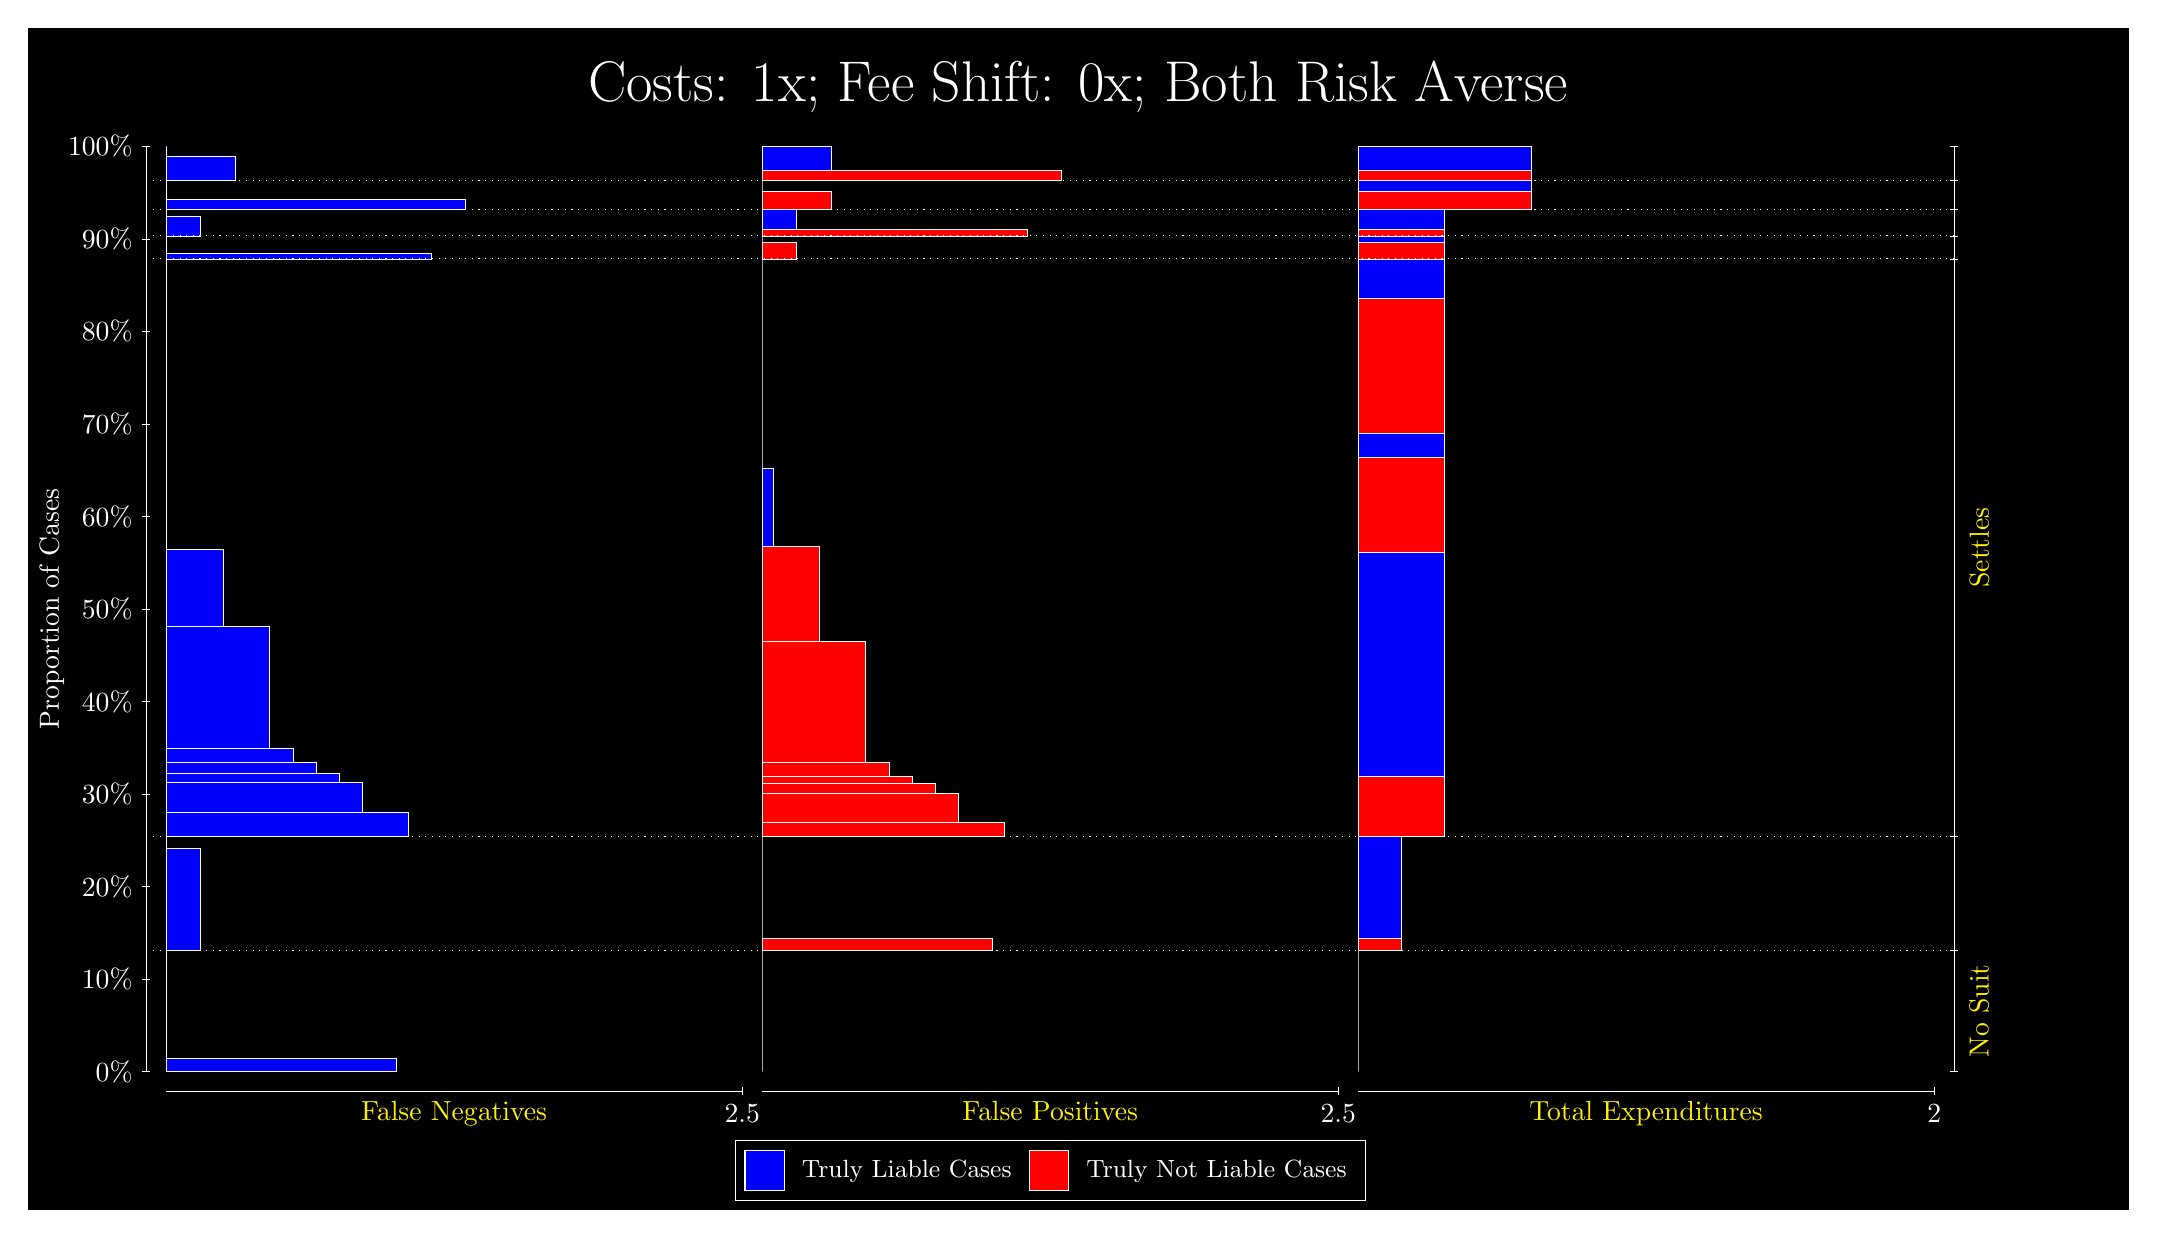
\begin{tikzpicture}
\draw[fill=black] (0,0) rectangle (26.667,15);
\draw[text=white] (0,13.5) rectangle (26.667,15) node[midway] {\huge Costs: 1x; Fee Shift: 0x; Both Risk Averse};
\draw[white, very thin] (1.5,1.75) -- (1.5,13.5);
\node[rotate=90, text=white, anchor=center] at (0.3, 7.625) {Proportion of Cases};
\draw[white, very thin] (1.45,1.75) -- (1.55,1.75);
\node[text=white, anchor=east] at (1.45, 1.75) {0\%};
\draw[white, very thin] (1.45,2.925) -- (1.55,2.925);
\node[text=white, anchor=east] at (1.45, 2.925) {10\%};
\draw[white, very thin] (1.45,4.1) -- (1.55,4.1);
\node[text=white, anchor=east] at (1.45, 4.1) {20\%};
\draw[white, very thin] (1.45,5.275) -- (1.55,5.275);
\node[text=white, anchor=east] at (1.45, 5.275) {30\%};
\draw[white, very thin] (1.45,6.45) -- (1.55,6.45);
\node[text=white, anchor=east] at (1.45, 6.45) {40\%};
\draw[white, very thin] (1.45,7.625) -- (1.55,7.625);
\node[text=white, anchor=east] at (1.45, 7.625) {50\%};
\draw[white, very thin] (1.45,8.8) -- (1.55,8.8);
\node[text=white, anchor=east] at (1.45, 8.8) {60\%};
\draw[white, very thin] (1.45,9.975) -- (1.55,9.975);
\node[text=white, anchor=east] at (1.45, 9.975) {70\%};
\draw[white, very thin] (1.45,11.15) -- (1.55,11.15);
\node[text=white, anchor=east] at (1.45, 11.15) {80\%};
\draw[white, very thin] (1.45,12.325) -- (1.55,12.325);
\node[text=white, anchor=east] at (1.45, 12.325) {90\%};
\draw[white, very thin] (1.45,13.5) -- (1.55,13.5);
\node[text=white, anchor=east] at (1.45, 13.5) {100\%};

\draw[white, very thin] (24.457,1.75) -- (24.457,13.5);
\draw[white, very thin] (24.407,1.75) -- (24.507,1.75);
\node[anchor=west] at (24.407, 1.75) {};
\draw[white, very thin] (24.407,3.29) -- (24.507,3.29);
\node[anchor=west] at (24.407, 3.29) {};
\draw[white, very thin] (24.407,4.7393) -- (24.507,4.7393);
\node[anchor=west] at (24.407, 4.7393) {};
\draw[white, very thin] (24.407,12.071) -- (24.507,12.071);
\node[anchor=west] at (24.407, 12.071) {};
\draw[white, very thin] (24.407,12.363) -- (24.507,12.363);
\node[anchor=west] at (24.407, 12.363) {};
\draw[white, very thin] (24.407,12.697) -- (24.507,12.697);
\node[anchor=west] at (24.407, 12.697) {};
\draw[white, very thin] (24.407,13.063) -- (24.507,13.063);
\node[anchor=west] at (24.407, 13.063) {};
\draw[white, very thin] (24.407,13.5) -- (24.507,13.5);
\node[anchor=west] at (24.407, 13.5) {};

\draw[white, very thin, fill=blue] (1.75,1.75) rectangle (4.6775,1.9224);
\draw[white, very thin, fill=red] (1.75,1.9224) rectangle (1.75,3.29);
\draw[white, very thin, fill=blue] (1.75,3.29) rectangle (2.1891,4.5895);
\draw[white, very thin, fill=red] (1.75,4.5895) rectangle (1.75,4.7393);
\draw[white, very thin, fill=blue] (1.75,4.7393) rectangle (4.8239,5.0485);
\draw[white, very thin, fill=blue] (1.75,5.0485) rectangle (4.2384,5.4255);
\draw[white, very thin, fill=blue] (1.75,5.4255) rectangle (3.9457,5.5441);
\draw[white, very thin, fill=blue] (1.75,5.5441) rectangle (3.6529,5.6825);
\draw[white, very thin, fill=blue] (1.75,5.6825) rectangle (3.3602,5.8587);
\draw[white, very thin, fill=blue] (1.75,5.8587) rectangle (3.0674,7.3992);
\draw[white, very thin, fill=blue] (1.75,7.3992) rectangle (2.4819,8.3839);
\draw[white, very thin, fill=red] (1.75,8.3839) rectangle (1.75,12.071);
\draw[white, very thin, fill=blue] (1.75,12.071) rectangle (5.1167,12.147);
\draw[white, very thin, fill=red] (1.75,12.147) rectangle (1.75,12.363);
\draw[white, very thin, fill=blue] (1.75,12.363) rectangle (2.1891,12.609);
\draw[white, very thin, fill=red] (1.75,12.609) rectangle (1.75,12.697);
\draw[white, very thin, fill=blue] (1.75,12.697) rectangle (5.5558,12.829);
\draw[white, very thin, fill=red] (1.75,12.829) rectangle (1.75,13.063);
\draw[white, very thin, fill=blue] (1.75,13.063) rectangle (2.6283,13.368);
\draw[white, very thin, fill=red] (1.75,13.368) rectangle (1.75,13.5);
\draw[white, very thin, fill=red] (9.3189,1.75) rectangle (9.3189,3.1176);
\draw[white, very thin, fill=blue] (9.3189,3.1176) rectangle (9.3189,3.29);
\draw[white, very thin, fill=red] (9.3189,3.29) rectangle (12.246,3.4398);
\draw[white, very thin, fill=blue] (9.3189,3.4398) rectangle (9.3189,4.7393);
\draw[white, very thin, fill=red] (9.3189,4.7393) rectangle (12.393,4.9116);
\draw[white, very thin, fill=red] (9.3189,4.9116) rectangle (11.807,5.2885);
\draw[white, very thin, fill=red] (9.3189,5.2885) rectangle (11.515,5.4071);
\draw[white, very thin, fill=red] (9.3189,5.4071) rectangle (11.222,5.5021);
\draw[white, very thin, fill=red] (9.3189,5.5021) rectangle (10.929,5.6783);
\draw[white, very thin, fill=red] (9.3189,5.6783) rectangle (10.636,7.2188);
\draw[white, very thin, fill=red] (9.3189,7.2188) rectangle (10.051,8.4263);
\draw[white, very thin, fill=blue] (9.3189,8.4263) rectangle (9.4652,9.4111);
\draw[white, very thin, fill=blue] (9.3189,9.4111) rectangle (9.3189,12.071);
\draw[white, very thin, fill=red] (9.3189,12.071) rectangle (9.758,12.287);
\draw[white, very thin, fill=blue] (9.3189,12.287) rectangle (9.3189,12.363);
\draw[white, very thin, fill=red] (9.3189,12.363) rectangle (12.686,12.451);
\draw[white, very thin, fill=blue] (9.3189,12.451) rectangle (9.758,12.697);
\draw[white, very thin, fill=red] (9.3189,12.697) rectangle (10.197,12.931);
\draw[white, very thin, fill=blue] (9.3189,12.931) rectangle (9.3189,13.063);
\draw[white, very thin, fill=red] (9.3189,13.063) rectangle (13.125,13.195);
\draw[white, very thin, fill=blue] (9.3189,13.195) rectangle (10.197,13.5);
\draw[white, very thin, fill=red] (16.888,1.75) rectangle (16.888,3.1176);
\draw[white, very thin, fill=blue] (16.888,3.1176) rectangle (16.888,3.29);
\draw[white, very thin, fill=red] (16.888,3.29) rectangle (17.437,3.4398);
\draw[white, very thin, fill=blue] (16.888,3.4398) rectangle (17.437,4.7393);
\draw[white, very thin, fill=red] (16.888,4.7393) rectangle (17.986,5.5021);
\draw[white, very thin, fill=blue] (16.888,5.5021) rectangle (17.986,8.3419);
\draw[white, very thin, fill=red] (16.888,8.3419) rectangle (17.986,9.5495);
\draw[white, very thin, fill=blue] (16.888,9.5495) rectangle (17.986,9.8587);
\draw[white, very thin, fill=red] (16.888,9.8587) rectangle (17.986,11.575);
\draw[white, very thin, fill=blue] (16.888,11.575) rectangle (17.986,12.071);
\draw[white, very thin, fill=red] (16.888,12.071) rectangle (17.986,12.287);
\draw[white, very thin, fill=blue] (16.888,12.287) rectangle (17.986,12.363);
\draw[white, very thin, fill=red] (16.888,12.363) rectangle (17.986,12.451);
\draw[white, very thin, fill=blue] (16.888,12.451) rectangle (17.986,12.697);
\draw[white, very thin, fill=red] (16.888,12.697) rectangle (19.083,12.931);
\draw[white, very thin, fill=blue] (16.888,12.931) rectangle (19.083,13.063);
\draw[white, very thin, fill=red] (16.888,13.063) rectangle (19.083,13.195);
\draw[white, very thin, fill=blue] (16.888,13.195) rectangle (19.083,13.5);
\draw[white, dotted] (1.5,3.29) -- (24.457,3.29);
\draw[white, dotted] (1.5,4.7393) -- (24.457,4.7393);
\draw[white, dotted] (1.5,12.071) -- (24.457,12.071);
\draw[white, dotted] (1.5,12.363) -- (24.457,12.363);
\draw[white, dotted] (1.5,12.697) -- (24.457,12.697);
\draw[white, dotted] (1.5,13.063) -- (24.457,13.063);
\draw[white, very thin] (1.75,1.5) -- (9.0689,1.5);
\node[text=yellow, anchor=north] at (5.4094, 1.5) {False Negatives};
\draw[white, very thin] (9.0689,1.45) -- (9.0689,1.55);
\node[text=white, anchor=north] at (9.0689, 1.45) {2.5};

\draw[white, very thin] (9.3189,1.5) -- (16.638,1.5);
\node[text=yellow, anchor=north] at (12.978, 1.5) {False Positives};
\draw[white, very thin] (16.638,1.45) -- (16.638,1.55);
\node[text=white, anchor=north] at (16.638, 1.45) {2.5};

\draw[white, very thin] (16.888,1.5) -- (24.207,1.5);
\node[text=yellow, anchor=north] at (20.547, 1.5) {Total Expenditures};
\draw[white, very thin] (24.207,1.45) -- (24.207,1.55);
\node[text=white, anchor=north] at (24.207, 1.45) {2};

\node[text=yellow, centered, rotate=90] at (24.777, 2.52) {No Suit};

\node[text=yellow, centered, rotate=90] at (24.777, 8.4051) {Settles};





\draw (12.978300999999998,1.5) node[draw=none] (baseCoordinate) {};
\begin{scope}[align=center]
        \matrix[scale=0.5, draw=white, below=0.5cm of baseCoordinate, nodes={draw}, column sep=0.1cm]{
            \node[rectangle, draw, minimum width=0.5cm, minimum height=0.5cm, fill=blue] {}; &
            \node[draw=none, font=\small, text=white] (B) {Truly Liable Cases}; &
            \node[rectangle, draw, minimum width=0.5cm, minimum height=0.5cm, fill=red] {}; &
            \node[draw=none, font=\small, text=white] (B) {Truly Not Liable Cases}; \\
            };
\end{scope}

\end{tikzpicture}
\end{document}